\defverbatim[colored]\curltarsier{%
  \begin{lstlisting}[language=bash,tabsize=8,basicstyle=\ttfamily]
    curl -i -X POST -d '                      \
          command: "persistent_storage/write" \
          data:                               \
            amount: "100 MB"                  \
            files: 10                         \
          wave:                               \
            remains: 3                        \
            buddies: 3                        \
    ' kubernetes.dev:6666/exec
  \end{lstlisting}
}

\begin{frame}
	\titlepage
\end{frame}

\section*{Content}
		\begin{frame}
			\frametitle{Content}
			\tableofcontents
		\end{frame}

\section{About}
		\begin{frame}
			\frametitle{Assignment}
			\begin{itemize}
				\item Make yourself familiar with the Kubernetes system.
				\item Compare Kubernetes in different environments.
				\item Design and implement a set of applications to simulate real traffic.
				\begin{itemize}
					\item Load configuration files, SSL certificates and static resources.
					\item Use persistent storage.
					\item Raise controlled faults, deadlocks, segmentation faults.
					\item Simulate heavy CPU and RAM load.
					\item Log their own activity and reliably transfer the logs to the central log storage.
				\end{itemize}
			\end{itemize}
		\end{frame}

		\begin{frame}
			\frametitle{Technologies?}
			\begin{columns}
        \begin{column}{0.48\textwidth}
					\begin{block}{Kubernetes}
    				 is an open-source system for automating deployment, operations, and scaling of containerized applications. \cite{kubernetesio}
    			\begin{figure}[htb]
    				\begin{center}
    					
\includegraphics[height=60px]{img/kubernetes-logo.png}
    					  \caption{Kubernetes \cite{kubernetes-logo}}
    				\end{center}
    			\end{figure}
    			\end{block}
        \end{column}
        \begin{column}{0.48\textwidth}
          \begin{block}{Docker}
		  		  allows you to package an application with all of its dependencies into a standardized unit for software development. \cite{dockerio-whatisdocker}
            \begin{figure}[htb]
    				  \begin{center}
    					  
\includegraphics[height=60px]{img/docker-logo.png}
    					  \caption{Docker \cite{docker-logo}}
    				  \end{center}
    			  \end{figure}
			    \end{block}
        \end{column}
      \end{columns}
		\end{frame}
    
  \subsection*{Possible problems with Kubernetes in Seznam.cz}
    \begin{frame}
      \frametitle{Possible problems with Kubernetes in Seznam.cz}
      \begin{columns}
        \begin{column}{0.48\textwidth}
            \begin{itemize}
              \item Docker registry
              \item Secrets distribution
              \item Logging
              \item Security
              \item Monitoring
              \item Static content of websites
            \end{itemize}
          \end{column}  
          \begin{column}{0.48\textwidth}
            \begin{figure}[htb]
    				  \begin{center}
    					  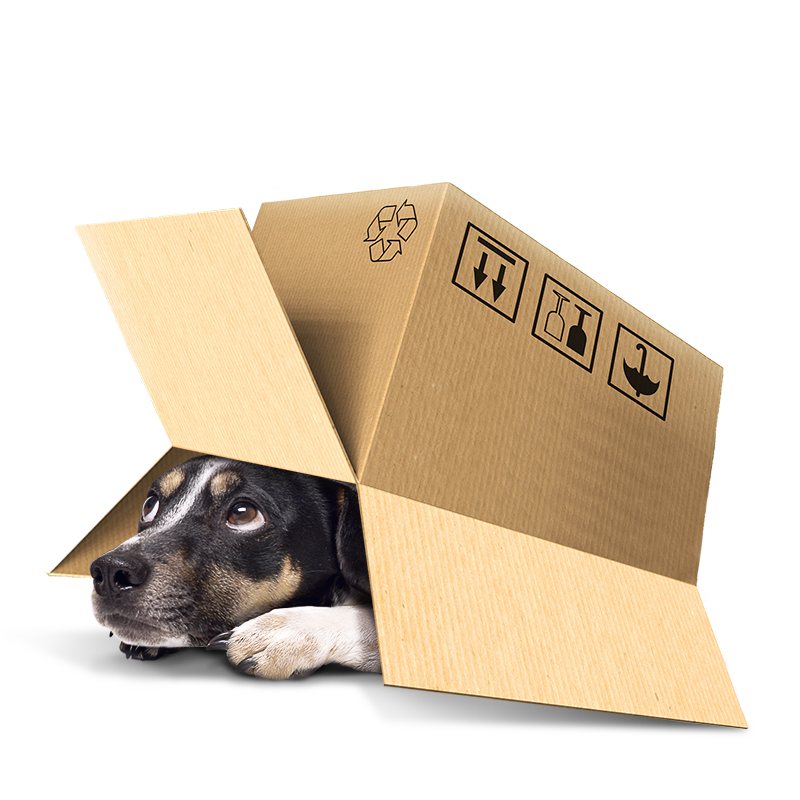
\includegraphics[width=\textwidth]{img/pes-krasty-seznam-15.png}
    					  \caption{Krasty \cite{krasty}}
    				  \end{center}
    			  \end{figure}
          \end{column}
        \end{columns}
    \end{frame}
    
    \begin{frame}
      \frametitle{Docker registry}
      \begin{figure}[htb]
			  \begin{center}
				  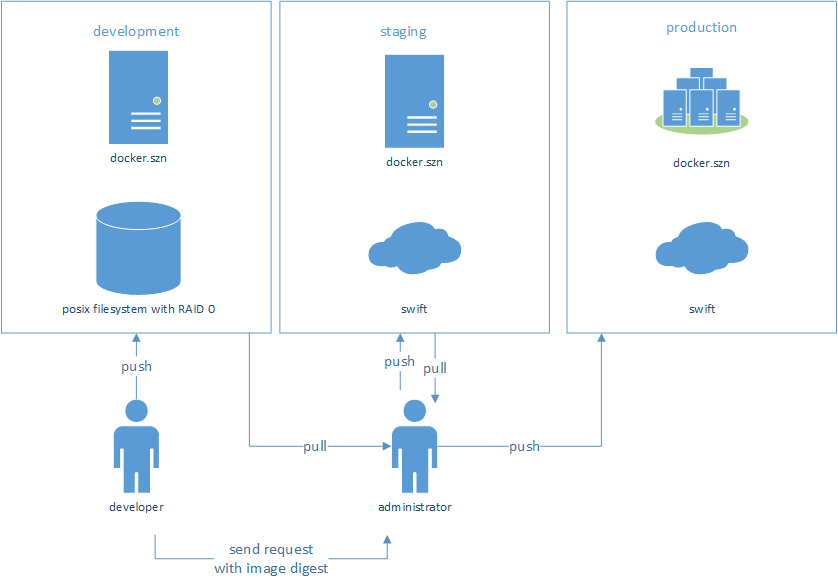
\includegraphics[width=1\textwidth]{img/docker-registry.png}
				  \caption{Docker registry}
			  \end{center}
		  \end{figure}
    \end{frame}
    
    \begin{frame}
      \frametitle{Logging I}
        \myheading{Debug logs}
          \begin{itemize}
            \item textual
            \item no need for 100\% reliability
          \end{itemize} 
        \myheading{Business logs}
          \begin{itemize}
            \item structured -- Apache Avro \cite{apache-avro}
            \item 100\% reliability
            \item not part of the thesis
          \end{itemize}
        \myheading{Third-party logs}
          \begin{itemize}
            \item system logs
            \item third-party applications (nginx mostly, \ldots) 
          \end{itemize}
          
        \textbf{Goal}: One solution to rule them all.
    \end{frame}
    
    \begin{frame}    
      \frametitle{Logging II}
        \myheading{Kafkalog}
          \begin{itemize}
            \item library for storing, rotating, compressing logs 
          \end{itemize}
        \myheading{Kafkafeeder}
          \begin{itemize}
            \item wrapper around Heka \cite{heka}
            \item sending messages from Kafkalog to Kafka \cite{kafka}
            \item with acknowledgement 
          \end{itemize} 
    \end{frame}        

    \begin{frame}
      \frametitle{Logging III}
        \myheading{Debug logs}
          \begin{itemize}
            \item Kafkalog handler to native loggers (Go Logrus \cite{logrus})
          \end{itemize} 
        \myheading{Business logs}
          \begin{itemize}
            \item additional library that uses Kafkalog
            \item not part of the thesis
          \end{itemize}
        \myheading{Third-party logs}
          \begin{itemize}
            \item simple application with various input interfaces (stdin, syslog, \ldots) 
            \item save to Kafkalog
            \item not part of the thesis             
          \end{itemize}
    \end{frame}

    \begin{frame}    
      \frametitle{Logging IV}
      \begin{figure}[htb]
			  \begin{center}
				  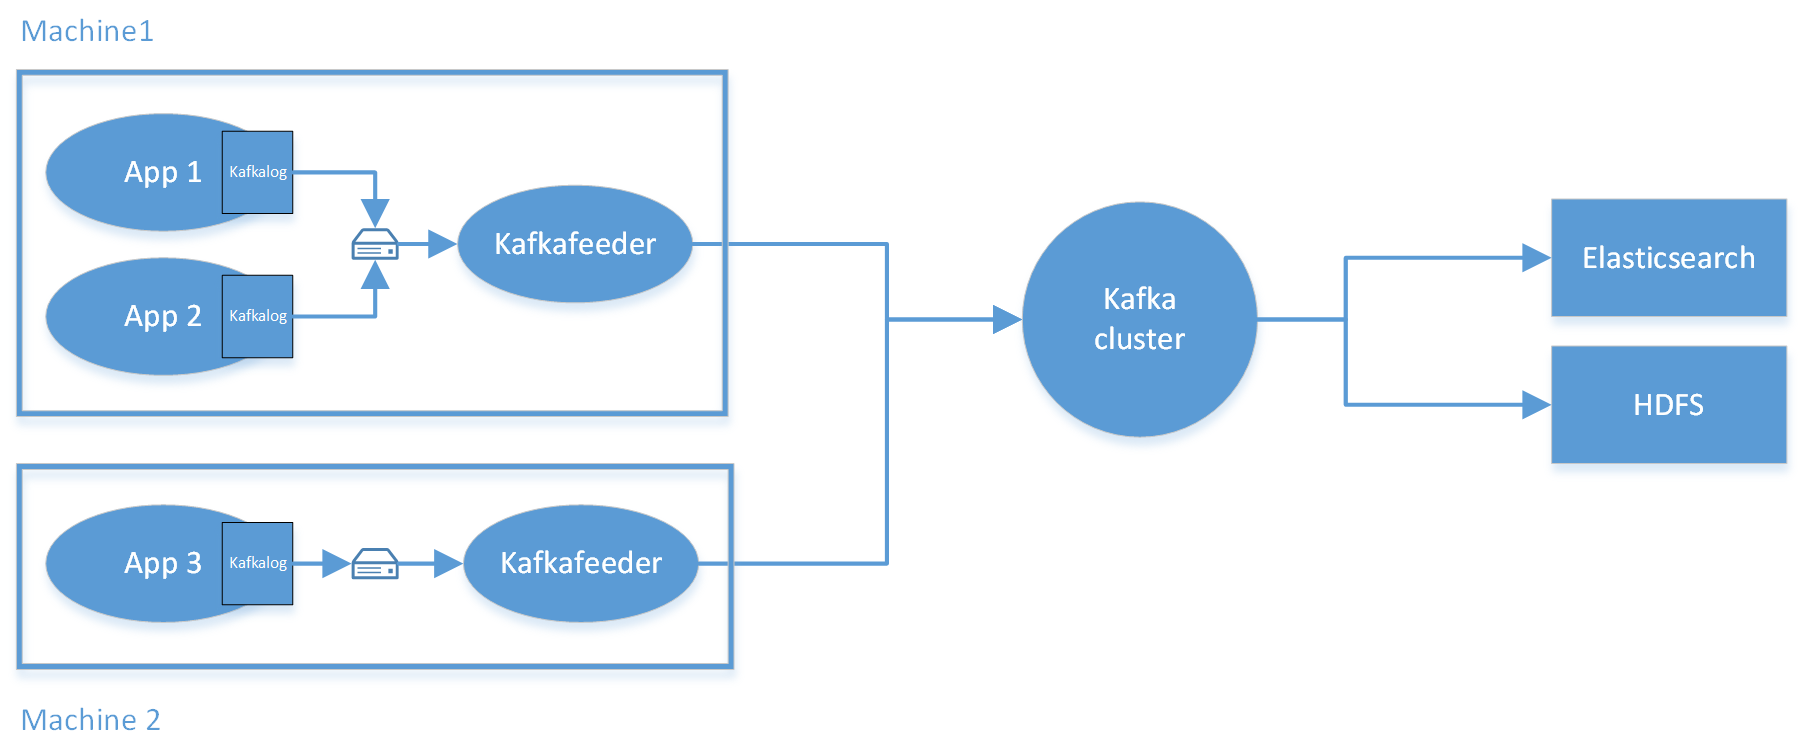
\includegraphics[width=\textwidth]{img/logging-flow.png}
				  \caption{Logging flow}
			  \end{center}
		  \end{figure}
         
    \end{frame}   

\section{Tarsier}    
    \begin{frame}    
      \frametitle{Tarsier I}
      \begin{columns}
        \begin{column}{0.48\textwidth}
          \begin{itemize}
            \item Testing application
            \item Modular
              \begin{itemize}
                \item \textcolor{myred}{Heavy load} -- Gobble RAM, Spin CPU  
                \item \textcolor{myred}{Faults} -- Deadlock, Segfault
                \item \textcolor{myred}{Net} -- Dial
                \item \textcolor{myred}{Persistent storage} -- Open, Read, Write
                \item \textcolor{myred}{Sleeping beauty} -- Sleep 
              \end{itemize}
          \end{itemize}        
         \end{column}
         \begin{column}{0.48\textwidth}    
          \begin{figure}[htb]
    			  \begin{center}
    				  
\includegraphics[width=0.9\textwidth]{img/tarsier.png}
    				  \caption{Tarsier \cite{tarsier-source}}
    			  \end{center}
    		  \end{figure}
         \end{column}
      \end{columns}
    \end{frame}
    
    \begin{frame}    
      \frametitle{Tarsier II}
         \curltarsier
    \end{frame}
    
    \begin{frame}    
      \frametitle{Tarsier III}
        \begin{figure}[htb]
  			  \begin{center}
  				  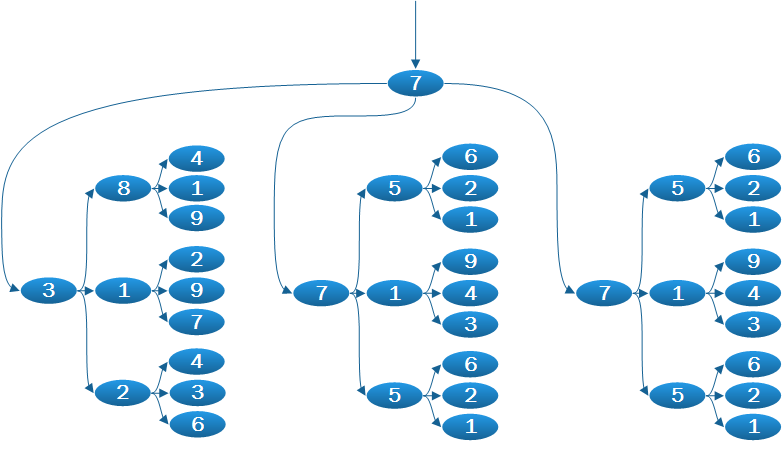
\includegraphics[width=0.95\textwidth]{img/tarsier-wave.png}
  				  \caption{Tarsier wave}
  			  \end{center}
  		  \end{figure}      
    \end{frame}

\section{Conclusion}
		\begin{frame}
			\frametitle{Output}				
			\url{https://github.com/sejvlond/master-thesis}
      
			\begin{description}[leftmargin=!,labelwidth=100px]
				\item[Tarsier] Application for testing Kubernetes cluster  
        \item[Kafkafeeder] Application that transfers logs to Kafka
        \item[Go kafkalog] Apache Kafka log format implementation in Go      
        \item[Kafkalog Logrus] Kafkalog hook to logrus
        \item[Heka] Some Heka adjustment for greater reliability 
        \item[Heka Kafkalog] Heka Splitter and Decored plugins that use go-kafkalog
        \item[Kubernetes testing] Support scripts for testing Kubernetes
        \item[Go Ultimate server] Simple Go server for benchmarking
        \item[Python Ultimate server] Simple Python Tornado server for benchmarking
			\end{description}
		\end{frame}

		\begin{frame}
			\frametitle{Benefits}				
			\bigskip
			\begin{enumerate}
				\item Kubernetes
        \item Docker
				\item Golang
        \item Kafka
				\item Heka
        \item Fluentd
        \item Logstash
			\end{enumerate}
		\end{frame}

		\begin{frame}
			\frametitle{Acknowledgements}
      \begin{columns}
        \begin{column}{0.48\textwidth}
    			\begin{itemize}
    				\item Ing. Jan Baier 
    				\item Ing. Tomáš Kukrál
    				\item David Bouček
            \item Martin Stružský
            \item Seznam.cz, a.s. 
    			\end{itemize}
          \end{column}  
          \begin{column}{0.48\textwidth}
            \begin{figure}[htb]
    				  \begin{center}
    					  
\includegraphics[width=\textwidth]{img/pes-krasty-seznam-13.png}
    					  \caption{Krasty \cite{krasty}}
    				  \end{center}
    			  \end{figure}
          \end{column}
        \end{columns}
		\end{frame}

		\begin{frame}[t,allowframebreaks]
			\frametitle{References}
				\bibliographystyle{iso690}
        \bibliography{references}
		\end{frame}

\section{Discussion}
		\begin{frame}
			\begin{center}
				\vspace*{1cm}
				{\bf Thank you for your attention}\\
				\vspace*{2cm}
				{\bf\Large \FirstName{} \LastName{}}\\
				{\tt \Email}
				\vspace*{1cm}
			\end{center}
			\vfill
		\end{frame}

\appendix
	\section{Opponent}
			\begin{frame}
				\begin{block}{Question}
					Why did you chose Kafkafeeder instead of native Docker's log drivers?
				\end{block}
				\begin{exampleblock}{Answer}<2->
          Docker's log drivers for container standard output \cite{docker-logs}
					\begin{description}	
            \item<2-> [json-file] JSON messages to file. \visible<3->{\xcancel{Kafka}}
            \item<4-> [syslog] to syslog. \visible<5->{\xcancel{Kafka, 1 kB}}
            \item<6-> [journald] to journald. \visible<7->{\xcancel{systemd}}
            \item<8-> [gelf] to a GELF endpoint likeGraylog or Logstash. \visible<9->{\xcancel{Graylog cluster, Logstash}}
            \item<10-> [fluentd] to fluentd (forward input). \visible<11->{\bf\textcolor{mygreen}{possible for debug logs}}
            \item<12-> [awslogs] to Amazon CloudWatch Logs. \visible<13->{\xcancel{Amazon CloudWatch}}
            \item<14-> [splunk] to splunk using HTTP Event Collector. \visible<15->{\xcancel{Splunk Cloud}}
            \item<16-> [etwlogs] ETW logging driver on Windows. \visible<17->{\xcancel{Windows}} 
            \item<18-> [gcplogs] to Google Cloud Logging. \visible<19->{\xcancel{Google Cloud}}
					\end{description}
				\end{exampleblock}
			\end{frame}
      
      \begin{frame}
				\frametitle{fluentd}
        \begin{figure}[htb]
    			\begin{center}
  					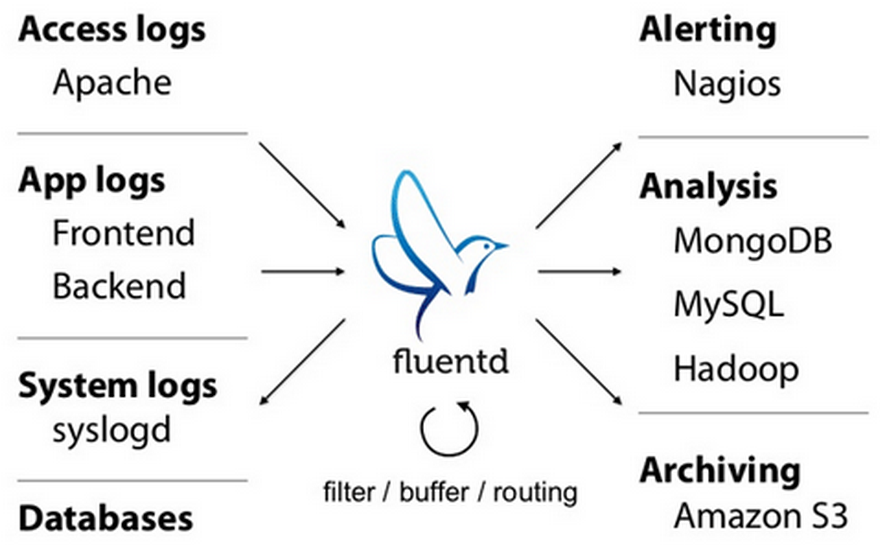
\includegraphics[width=0.8\textwidth]{img/fluentd-architecture.png}
  					  \caption{fluentd \cite{fluentd-architecture}}
  				\end{center}
  			\end{figure}
			\end{frame}
      
\section*{End}
		\begin{frame}
			\begin{center}
				\vspace*{1cm}
				{\bf Thank you for your attention}\\
				\vspace*{2cm}
				{\bf\Large \FirstName{} \LastName{}}\\
				{\tt \Email}
				\vspace*{1cm}
			\end{center}
			\vfill
		\end{frame}      